 \documentclass[11pt]{article}

\usepackage[english]{babel}
\usepackage[margin=1in]{geometry}

% Math/Greek packages
\usepackage{amssymb,amsmath,amsthm, mathtools} 
\usepackage{algorithm, algorithmic}
\usepackage{upgreek, siunitx}
\usepackage{setspace}

% Graphics/Presentation packages
\usepackage{multirow}
\usepackage{graphicx}
\usepackage{cancel}
\usepackage{tabulary, enumitem, array}
\usepackage{xparse,mleftright,tikz}
\usepackage{physics}

% Misc packages
\usepackage{fancyhdr}


\usepackage[export]{adjustbox}

\usepackage{esint}

\sisetup{locale=US,group-separator = {,}}
\usepackage[colorlinks=true, allcolors=blue]{hyperref}


\begin{document}

\title{PHSX 462: HW08}
\author{William Jardee}
\maketitle


\section*{Griffiths 8.1}
\begin{enumerate}[label=\alph*)]
\item We are given a potential of $V(x) = \alpha \abs{x}$, and that we need to use the Gaussian guess, $\displaystyle{\psi(x) = \left(\frac{2b}{\pi}\right)^{1/4}e^{-bx^2}}$, where our variation parameter is $b$. The total Hamiltonian will be the combination of kinetic with potential:
\[H = -\frac{\hbar^2}{2m}\pdv[2]{x} + \alpha\abs{x} \, .\]
Doing the kinetic term first, we get (skipping some steps because this is far from the first time doing this calculation):
\begin{align*}
\ev{T} & = -\frac{\hbar^2}{2m}\left(\frac{2b}{\pi}\right)^{1/2}\int_{-\infty}^\infty e^{-bx^2}\dv[2]{x}e^{-bx^2}\dd{x}\\
& = -\frac{\hbar^2}{2m}\left(\frac{2b}{\pi}\right)^{1/2}2b\int_{-\infty}^\infty \left(-e^{-2bx^2} + 2bx^2e^{2bx^2}\right)\dd{x}\\
& = -\frac{2\hbar^2 b}{m}(2b)^{1/2}\left(-\frac{1}{2\sqrt{2b}} + \frac{1}{4\sqrt{2b}}\right)\\
& = \frac{\hbar^2 b}{2m} \, .
\end{align*}
This is also the value that is derived in the book. For the potential:
\begin{align*}
\ev{V} & = \left(\frac{2b}{\pi}\right)^{1/2} \alpha \int_{-\infty}^\infty e^{-2bx^2} \abs{x} \dd{x}\\
& = 2\left(\frac{2b}{\pi}\right)^{1/2} \alpha \int_0^\infty e^{-2bx^2} x \dd{x} \\
 & = \frac{\alpha}{2b}\left(\frac{2b}{\pi}\right)^{1/2} = \frac{\alpha}{\sqrt{2b\pi}} \, . 
\end{align*}
Putting the two of these together we get
\[\ev{H} = \frac{\hbar^2 b}{2m} + \frac{\alpha}{\sqrt{2b\pi}} \, . \]

To find the $b$ that minimizes the energy we need to find where the derivative is zero, i.e.
\[\pdv{\ev{H}}{b} = \frac{\hbar^2}{2m} - \frac{1}{2}\frac{\alpha}{\sqrt{2\pi}}b^{-3/2} = 0\]
\[b = \left(\frac{\hbar^2}{m}\frac{\sqrt{2\pi}}{\alpha}\right)^{2/3} = \left(\frac{m\alpha}{\hbar^2\sqrt{2\pi}}\right)^{2/3} \, .\]
Substituting this back into our equation for the $\ev{H}$, the upper-bound of the minimum energy is
\begin{align*}
E_\text{gs} \leq \ev{H}_\text{min} & = \frac{\hbar^2}{2m}\left(\frac{m\alpha}{\hbar^2 \sqrt{2\pi}}\right)^{2/3} + \frac{\alpha}{\sqrt{2\pi}}\left(\frac{\hbar^2 \sqrt{2\pi}}{m\alpha}\right)^{1/3}\\
E_\text{gs} & \leq \boxed{ \, \frac{3}{2}\left(\frac{\alpha^2 \hbar^2}{2\pi m}\right)^{1/3} \,} \, . 
\end{align*}

\item Now, let's do the same calculation with $\displaystyle{V(x) = \alpha x^4}$. The $\ev{T}$ will be the same, so we just need to do the potential calculation:
\begin{align*}
\ev{V} & = \abs{A}^2 \int_{-\infty}^\infty e^{-bx^2}\alpha x^4 e^{-bx^2}\dd{x}\\
& = \left(\frac{2b}{\pi}\right)^{1/2} 2\alpha \int_0^\infty e^{-2bx^2}x^4\dd{x}\\
& = \frac{3\alpha}{16b^2} \, . 
\end{align*}
This give 
\[\ev{H} = \frac{\hbar^2 b}{2m} + \frac{3\alpha}{16b^2} \, . \]

Minimizing with respect to $b$, just like in part a:
\[\pdv{\ev{H}}{b} = \frac{\hbar^2}{2m} - \frac{3\alpha}{8b^3}\]
\[b = \left(\frac{3\alpha m}{4\hbar^2}\right)^{1/3} \, . \]
Substituting this back in, and simplifying gives
\begin{align*}
E_\text{gs} \leq \ev{H}_\text{min} & = \frac{\hbar^2}{2m}\left(\frac{3\alpha m}{4\hbar^2}\right)^{1/3} + \frac{3\alpha}{16}\left(\frac{4\hbar^2}{3\alpha m}\right)^{2/3}\\
E_\text{gs} & \leq \boxed{\, \frac{3}{4}\left(\frac{3\alpha \hbar^4}{4m^2}\right)^{1/3} \, }\, .	 
\end{align*}
\end{enumerate}

%--------------------------------------------------------------------------------
\newpage

\section*{Question 2}
There is not many comments to be made on this one other than to show that it is normalized:
\begin{align*}
\abs{\psi(\vec{r}_1, \vec{r}_2)}^2 & = \left(\frac{Z^3}{\pi a_0^3}\right)^2 \int_0^{2\pi}\int_0^\pi \int_0^\infty e^{-2Zr_1/a_0}r_1^2 \sin(\theta_1)\dd{r_1}\dd{\theta_1}\dd{\phi_1}\\
& \hspace{6em} \times \int_0^{2\pi}\int_0^\pi \int_0^\infty e^{-2Zr_21/a_0}r_2^2 \sin(\theta_2)\dd{r_2}\dd{\theta_2}\dd{\phi_2}\\
& = \left(\frac{Z^3}{\pi a_0^3}\right)^2 \left(4\pi\right)^2 \left[\int_0^\infty e^{-2Zr/a_0} r^2 \dd{r}\right]^2\\
& = \left(\frac{4Z^3}{a_0^3}\right)^2 \left(2! \left(\frac{a_0}{2Z}\right)^3\right)^2 = \left(\frac{4Z^3}{a_0^3}\right)\left(\frac{a_0^3}{4Z^3}\right)^2 = 1 \, . \qquad \checkmark
\end{align*}

%--------------------------------------------------------------------------------
\newpage

\section*{Griffiths 8.4a}
\begin{enumerate}[label=\alph*)]
\item It is given that $\braket{\psi}{\psi_\text{gs}} = 0$. That means that is we expand the wavefunction according to the energy levels (where the ground state corresponds to $n = 0$)
\[\psi = \sum_{n=1} c_n\psi_n \, . \]
Then
\begin{align*}
\ev{H} & = \ev{H}{\psi} = \ev{\sum_{n=1} c_n\psi_n}{\psi} = \sum_{n=1}\abs{c_n}^2 \ev{\psi_n}{H}\\
& = \sum_{n=1}\abs{c_n}^2 E_n \geq E_1 \, . 
\end{align*}
\hfill $\blacksquare$
\end{enumerate}

%--------------------------------------------------------------------------------
\newpage

\section*{Griffiths 8.30a, b}
\begin{enumerate}[label=\alph*)]
\item This is another ``just derive question". So, let's just do it:
\begin{align*}
\pdv{c_j^*} \varepsilon & = \pdv{c_j^*}\left[\left(\sum_{m \, n} c^*_m H_{mn} c_n\right)\left(\sum_n \abs{c_n}\right)^{-1}\right]\\
& = \left(\sum_{n}H_{jn} c_n\right)\left(\sum_{n}\abs{c_n}^2\right)^{-1} - \left(\sum_{m \, n} c^*_m H_{mn} c_n\right)\left(\sum_n \abs{c_n}\right)^{-2}c_j \, . 
\end{align*}
Setting this equal to zero gives
\begin{align*}
\left(\sum_{n}H_{jn} c_n\right)\left(\sum_{n}\abs{c_n}^2\right)^{-1} & = \left(\sum_{m \, n} c^*_m H_{mn} c_n\right)\left(\sum_n \abs{c_n}\right)^{-2}c_j\\
\sum_{n}H_{jn} c_j = \frac{\sum_{m \, n}c_m^* H_{mn}c_n}{\sum_{n}\abs{c_n}^*} c_j = \varepsilon c_j \, .
\end{align*}
So,
\begin{equation}
\boxed{\sum_{n}H_{jn} c_j = \varepsilon c_j}
\label{eq:1}
\end{equation}
\item
The derivation is nearly identical to the previous part:
\begin{align*}
\pdv{c_j} \varepsilon & = \pdv{c_j}\left[\left(\sum_{m \, n} c^*_m H_{mn} c_n\right)\left(\sum_n \abs{c_n}\right)^{-1}\right]\\
& = \left(\sum_{m}c_m H_{mj}\right)\left(\sum_{n}\abs{c_n}^2\right)^{-1} - \left(\sum_{m \, n} c^*_m H_{mn} c_n\right)\left(\sum_n \abs{c_n}\right)^{-2}c_j^* \, . 
\end{align*}
Setting this equal to zero gives
\begin{align*}
\left(\sum_{m}c_m H_{mj}\right)\left(\sum_{n}\abs{c_n}^2\right)^{-1} & = \left(\sum_{m \, n} c^*_m H_{mn} c_n\right)\left(\sum_n \abs{c_n}\right)^{-2}c_j^*\\
\sum_{m}c_m H_{mj}= \frac{\sum_{m \, n}c_m^* H_{mn}c_n}{\sum_{n}\abs{c_n}^*} c_j^* = \varepsilon c_j^* \, .
\end{align*}
So,
\begin{equation}
\boxed{\sum_{m}c_m H_{mj} = \varepsilon c_j^*}
\label{eq:2}
\end{equation}

To show that this is redundant to equation~\ref{eq:1}, let's take the complex conjugate of both sides of equation~\ref{eq:2}:
\begin{align*}
\left[\sum_{m}c_m H_{mj}\right]^* &= \left[\varepsilon c_j^*\right]^*\\
\sum_{m} c_m^* H_{mj}^* & = \varepsilon^* \left(c_j^*\right)^*\\
\sum_{m} H_{jm} c_m^* & = \varepsilon^* c_j \, .
\end{align*}
The third line is justified by the fact that $H$ is Hermitian, so $H^\dagger = H$ and $\varepsilon$ is defined off of real quantities, so the complex conjugate will be equivalent to it. Since we got back to equation~\ref{eq:1} without introducing any new information, equation~\ref{eq:2} is redundant.
\end{enumerate}

%--------------------------------------------------------------------------------
\newpage

\section*{Question 5}
Setting up the normalization requirement and following the trail:
\begin{align*}
\abs{\psi_\pm(\vec{r}_1, \vec{r}_2)}^2 & = \left(A_\pm \left[\psi_0(\vec{r}_1)\psi_0(\vec{r}_2^\prime)\pm \psi_0(\vec{r}_1^\prime)\psi_0(\vec{r}_2)\right]\right)\left(A_\pm \left[\psi_0(\vec{r}_1)\psi_0(\vec{r}_2^\prime)\pm \psi_0(\vec{r}_1^\prime)\psi_0(\vec{r}_2)\right]\right)\\
1 & = \abs{A_\pm}^2 \left(\left[\psi_0(\vec{r}_1)\psi_0(\vec{r}_2^\prime)\right]\left[\psi_0(\vec{r}_1)\psi_0(\vec{r}_2^\prime)\right]^* \pm \left[\psi_0(\vec{r}_1)\psi_0(\vec{r}_2^\prime)\right]\left[\psi_0(\vec{r}_1^\prime)\psi_0(\vec{r}_2^)\right] \right.\\
& \hspace{4em}\left. \pm \left[\psi_0(\vec{r}_1^\prime)\psi_0(\vec{r}_2)\right]\left[\psi_0(\vec{r}_1)\psi_0(\vec{r}_2^\prime)\right] + \left[\psi_0(\vec{r}_1^\prime)\psi_0(\vec{r}_2)\right]\left[\psi_0(\vec{r}_1^\prime)\psi_0(\vec{r}_2)\right]\right)\\
& \text{Recognizing that } \psi_0 = \psi_0^* \text{ thus } \abs{\psi_0}^2 = \psi_0^2 = 1\\
& = \abs{A_\pm}^2 \left(\abs{\psi_0(\vec{r}_1)}^2\abs{\psi_0(\vec{r}_2^\prime)}^2 + \abs{\psi_0(\vec{r}_1^\prime)}^2\abs{\psi_0(\vec{r}_2)}^2 \pm 2 \psi_0(\vec{r}_1)\psi_0(\vec{r}_1^\prime)\psi_0(\vec{r}_2)\psi_0(\vec{r}_2^\prime)\right)\\
& = \abs{A_\pm}^2\left(1 + 1 \pm \underbrace{\psi_0(\vec{r}_1)\psi_0(\vec{r}_1^\prime)}_I\underbrace{\psi_0(\vec{r}_2)\psi_0(\vec{r}_2^\prime)}_I \right)\\
& = \abs{A_\pm}^2\left(2 \pm 2I^2\right)
\end{align*}
Solving for $A$ gives
\[\abs{A_\pm} = \frac{1}{\sqrt{2(1 \pm I^2)}} \, .\]

Solving for the value of the crossover integral, $I$
\begin{align*}
I & = \frac{1}{\pi a^3}\int e^{-r/a}e^{-r^\prime /a} \, \dd[3]{\vec{r}} = \frac{1}{\pi a^3}\int e^{-(r+r^\prime)/a}\dd[3]{\vec{r}}\\
& = \frac{1}{\pi a^3} \int e^{-r/a}e^{-\sqrt{r^2 + R^2 - 2rR \cos(\theta)}/a}r^2 \sin(\theta)\dd{r}\dd{\theta}\dd{\phi}
\end{align*}
The $\phi$ integral is trivially $2\pi$. Doing the $\theta$ integral with a $\displaystyle{u = \sqrt{r^2 + R^2 - 2rR \cos(\theta)}}$
\begin{align*}
\frac{1}{\pi a^3} & \int_\abs{r-R}^{r+R} e^{-u/a} \frac{1}{rR} u \dd{u}\\
\frac{1}{\pi a^2 rR} & \left[e^{-(r+R)/a}(r+R+a) - e^{-\abs{r-R}/a}(\abs{r-R} + a)\right] \, .
\end{align*}

Now to do the $r$ integral:
\begin{align*}
I & = -\frac{2 \pi}{\pi a^2 R} \int_0^\infty e^{-r/a} \left(e^{-(r-R)/a}(r+R+a) - e^{\abs{r-R}/a}(\abs{r-R} + a)\right)\frac{1}{r}r^2\dd{r}
\end{align*}
Splitting the integral on absolute value gives
\begin{align*}
I& = \frac{2}{a^2 R} \left[-e^{-R/a}\int_0^\infty (r+R+a)e^{-2r/a} r\dd{r} \right.\\
& \hspace{6em} \left.+ e^{-R/a}\int_0^R (R+r+a)r\dd{r} + e^{R/a}\int_R^\infty (r-R+a)e^{-2r/a}r\dd{r}\right]
\end{align*}
Doing the third integral as a scratch work and filling it in gives
\begin{align*}
I & = \frac{2}{a^2 R}\left[-e^{-R/a}\left[\left(2! \left(\frac{a}{2}\right)^3\right) + (R+a)\left( 1! \left(\frac{a}{2}\right)^2\right)\right] + e^{-R/a}\left(-\frac{1}{3}R^3 + (R+a)\frac{1}{2}R^2\right) \right.\\
& \hspace{6em}\left. + e^{R/a}\frac{e^{-2R/a}}{4}a^2(2a+3R)\right]\\
& = \frac{2}{6a^2 R}e^{-R/a}\left[-3a^3 - 3Ra^2 - 3a^3 - 4R^3 + 6R^3 + 6aR^2 + 6a^3 + 9a^2R\right]\\
& = \frac{1}{6} e^{-R/a}\left[6 + 6\frac{R}{a} + 2\frac{R^2}{a^2}\right]\\
I & = e^{-R/a}\left[1 + \frac{R}{a} + \frac{1}{3}\left(\frac{R}{a}\right)^2\right] \, . \qquad \checkmark
\end{align*}

%--------------------------------------------------------------------------------
\newpage

\section*{Question 6}

The answers to this question are given in Giffiths, so I will restate their solution and justify it. The bonding distance is at the equilibrium point, where the potential reaches a minimum. In figure~\ref{fig:6.1} the red circle indicates this. The value is about $\boxed{\, 1.6 \text{ the Bohr radius}\,}$ (this is pretty close to the $1.4$ found from experiments). The singlet state (the bottom solid curve) has an energy of $\ev{H} \approx -2.2 \abs{E_1}$ and the triplet state (the top dashed curve) has an energy of $\ev{H} \approx -1.5\abs{E_1}$. The difference is these two value is 
\[\Delta \ev{H} \approx \boxed{\,-0.7 \, \abs{E_1}\,} = -0.7 \cdot 13.6 \text{eV} = 9.5 \text{eV} \, . \]
This is close to the $-10$ eV that the book states.

\begin{figure}[!ht]
\centering
	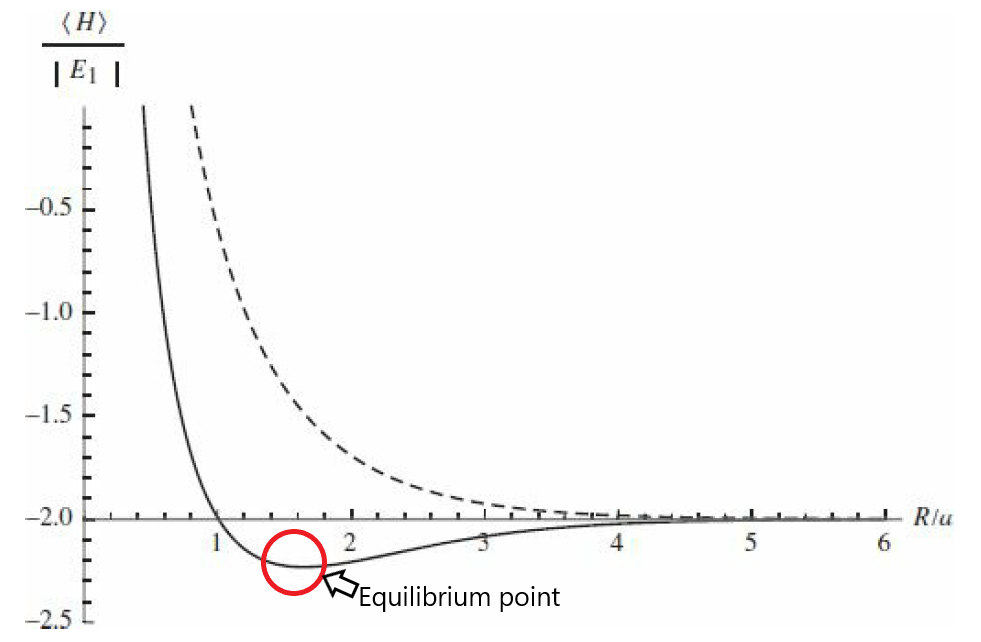
\includegraphics[width=0.9\linewidth]{phsx462_hw08_01.PNG}
	\caption{Figure 8.9 from Griffiths. The bottom solid line is the covalent bond energy from the singlet state. The top dashed is the bond energy from the triplet state. The rending of the text I have is slightly out of focus, so I apologize for the quality of the plot. }
	\label{fig:6.1}
\end{figure}


\end{document}
